\documentclass[preprint]{sigplanconf}
\usepackage{minted}
\usepackage{graphicx}

% The following \documentclass options may be useful:

% preprint      Remove this option only once the paper is in final form.
% 10pt          To set in 10-point type instead of 9-point.
% 11pt          To set in 11-point type instead of 9-point.
% numbers       To obtain numeric citation style instead of author/year.

\usepackage{amsmath}

\newcommand{\cL}{{\cal L}}

\begin{document}

\special{papersize=8.5in,11in}
\setlength{\pdfpageheight}{\paperheight}
\setlength{\pdfpagewidth}{\paperwidth}

\conferenceinfo{CONF 'yy}{Month d--d, 20yy, City, ST, Country}
\copyrightyear{20yy}
\copyrightdata{978-1-nnnn-nnnn-n/yy/mm}
\copyrightdoi{nnnnnnn.nnnnnnn}

% Uncomment the publication rights you want to use.
%\publicationrights{transferred}
%\publicationrights{licensed}     % this is the default
%\publicationrights{author-pays}

\titlebanner{banner above paper title}        % These are ignored unless
\preprintfooter{short description of paper}   % 'preprint' option specified.

\title{Polite programmers, write code with sentence case identifiers}
\subtitle{Subtitle Text, if any}

\authorinfo{Mircea Lungu}
           {University of Groningen}
           {i@mir.lu}
\authorinfo{Jan Kurs}
           {University of Bern}
           {jan@...}

\maketitle

\begin{abstract}

\noindent
TheJavaPeopleUseCamelCaseToSeparateWordsInTheirIdentifiers. 

\noindent
Pythonistas\_and\_their\_friends\_use\_underscore\_in\_their\_identifiers. 

\noindent
Polite programmers use sentence case to recall that code is prose.
\end{abstract}
\vspace {1cm}
\category{CR-number}{subcategory}{third-level}

\keywords
keyword1, keyword2

%!TEX root=../paper.tex


\section{Introduction}

Polite is an evolution of the Smalltalk programming language that aims to encourage developers to think more about their programs as prose. The main mechanism by which Polite does this is what we define here as sentence case identifiers -- a naming convention that allows spaces in identifier names. Polite illustrates that it is possible to embed spaces in identifier names while still storing and editing programs as text. 

Although spaces in identifiers have been used before in DSLs (e.g. Applescript, the Cucumber testing framework, Inform 7) or COBOL, the feature is unusual for a general purpose object-oriented text-based programming language. We suspect that the main reason for this is historical: spaces allow the scanner to easily tokenize the text in a traditional compiler backend architecture. We believe howevr, that easing the job of the programmer should come before easing the job of the scanner. 

If a syntax like that of Polite will encourage developers to think more about their programs as prose, and thus maybe work just a little bit harder towards writing more beautiful and readable code, it would be worth investigating using sentence case identifiers in other languages. Indeed, since software developers spend the largest part of their time reading code rather than writing it, even the smallest increase in code readability is to be fought for and cherished.
Some readers will argue that nobody in their right mind would use such long identifiers as we illustrated in the abstract. For those readers, we report three method names that can be found in popular open source programs written in one of the most popular programming languages at the moment: 


\begin{minted}[bgcolor=lbcolor]{text}
// nakedobjects-4.0.0
whenCallEnsureThatContextOverloadedShouldThrowIll
egalThreadStateExceptionUsingSuppliedMessage 

// aspectj-1.6.9
getPointcutParserSupportingSpecifiedPrimitivesAnd
UsingSpecifiedClassLoaderForResolution 

// maven-3.0
disabledtestResolveCorrectDependenciesWhenDiffer
entDependenciesOnNewestVersionReplaced 
\end{minted}





%!TEX root=../paper.tex

\section{Illustrating the Syntax}

Polite, the language that we propose here, is a variant of Smalltalk that started as an experiment in syntax. It is derived from Smalltalk to which we add sentence case identifiers, first class functions, and the concept of a program. 

In Smalltalk the syntax for sending a message with no arguments to an object is very elegantly implemented by simply separating the two entities with a space. If we have an object that represents a hero in a role playing game, we could send a message to it like this: 

\begin{minted}{Python} 
politeHero rechargeEnergy.
\end{minted} 

In order to replace identifiers with sentences, we need to make sure that our language grammar allows for the code to be parsed unambiguously. Since we allow space in the name of identifiers, we cannot use it anymore to separate the object and the message. Instead, in Polite, we use a comma to separate an agent’s name from the message that is sent to it, as in the sentence “Alfred, get the Batwing ready”. The previous code snippet becomes thus: 

\begin{minted}{Python} 
polite hero, recharge energy. 
\end{minted}

Note that all the words in an identifier including the spaces but excluding the last space are relevant for the identity of the identifier.

For the Smalltalkers out there, this smells like profanity, since `,’ is usually used as the concatenation operator for strings and other collections. It is worth noting though, that such a sentiment is misplaced since `,’ is not part of the core language, but rather is a simple message implemented in the Collection class. In Polite, we consequently overloaded the `+’ operator to take over the responsibilities of `,’.

The Smalltalk grammar does not provide productions for programs or classes, since the programmer compiles a method at a time. We therefore introduce these productions to be able to write larger programs.


A simple class would thus look like this:
\newpage

% $\lstinputlisting[language=Python]{polite-hero.polite}



In the previous example we observe class and local variable declarations. This is another example where the original Smalltalk grammar has to be modified since the original separator between variable names used to be space. Now the separator is again `,’. However, we kept the pipe notation for variable declarations.

Since Polite allows the definition of first class functions we can implement new control structures like the one we have used in the fight with: method: 

\begin{minted}{Python}
while neither: [self, is dead] nor: [an enemy, is dead] do: [...] 
\end{minted}

Such ad-hoc control structures can often improve the readability of program text as other languages like Grace have also shown. In our example, to illustrate the difference in readability, we show the equivalent method for fight with: written here in traditional Smalltalk:

\begin{minted}{Smalltalk}
fightWith: anEnemy
((self isDead not) and: [anEnemy isDead not]) whileTrue: [
    self throwAPunchAt: theEnemy.
    theEnemy throwAPunchAt: self.
]
\end{minted}

The highlighted line of code will be hard to read for beginners [citation about control structures in St being hard in general for beginners] and could even be error prone for advanced developers.  shows the usefulness of having first class functions. Especially since the control structures of Smalltalk turn out to puzzle beginners [citation needed]. 

%!TEX root=../paper.tex

\section{Implementation}
Polite is implemented on top of Pharo Smalltalk and PetitParser is used to define its grammar as parsing expressions. The implementation can be found online. The code examples from this paper are fragments of a larger example that can also be found in the Polite image available online. 

\begin{figure}[h]
	\centering
	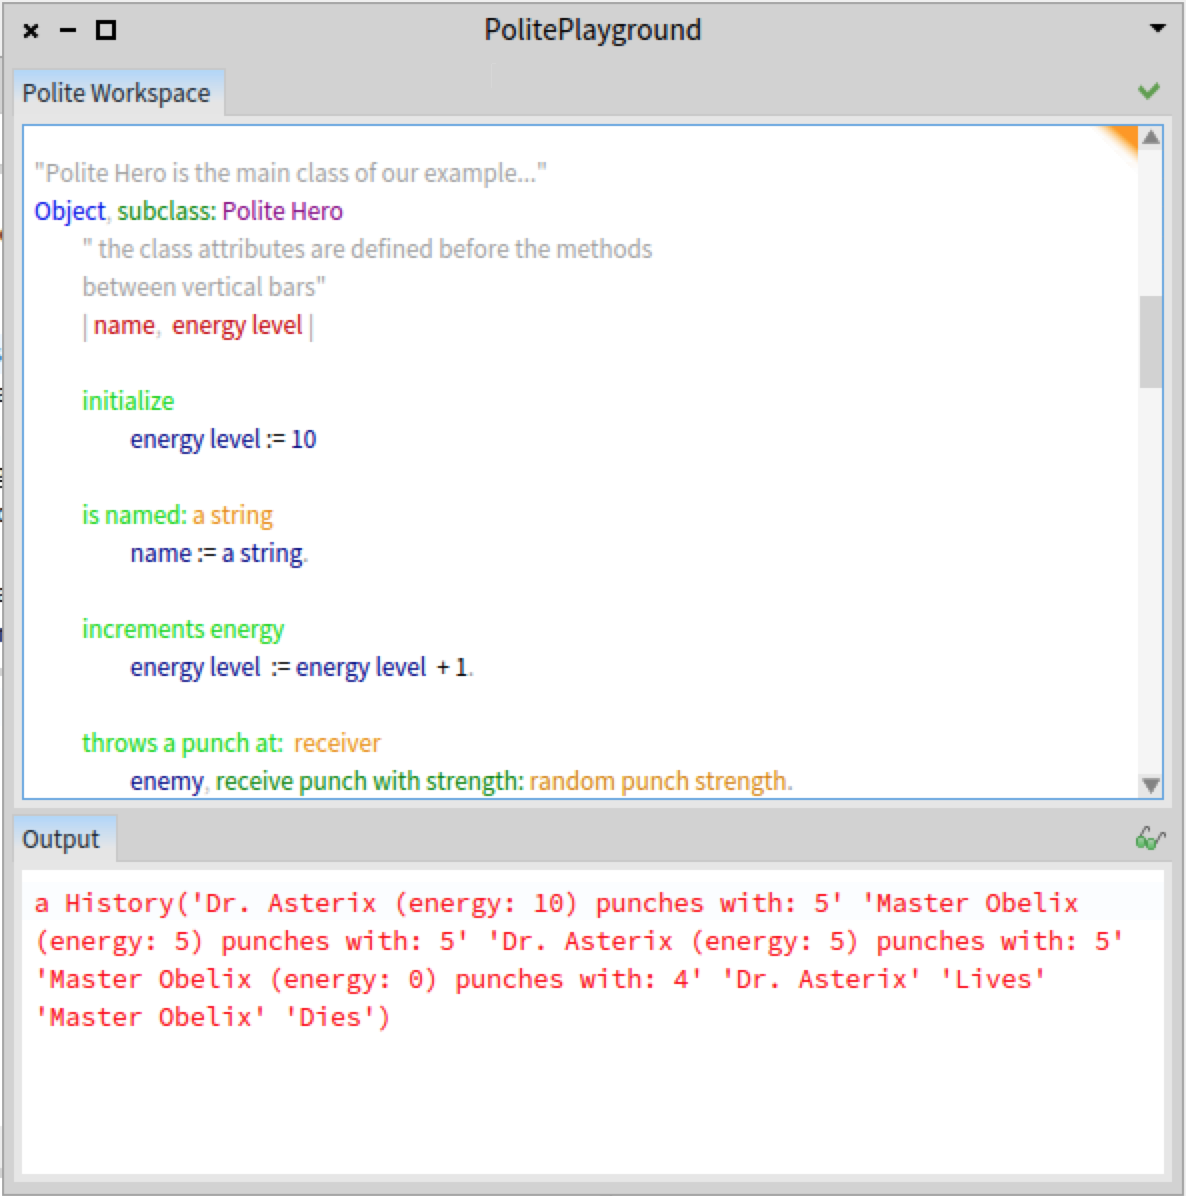
\includegraphics[width=0.5\textwidth]{images/playground.png}
	\caption{The Polite Playground provides a syntax highlighting code editor for Polite}
	\label{fig:figure1}
\end{figure}




\acks

We would like to thank Oscar Nierstrasz and Tijs van der Storm for feedback on earlier versions of this paper. We would like to thank our students T. Steinmann, 



% We recommend abbrvnat bibliography style.

\bibliographystyle{abbrvnat}

% The bibliography should be embedded for final submission.

\begin{thebibliography}{}
\softraggedright

\bibitem[Smith et~al.(2009)Smith, Jones]{smith02}
P. Q. Smith, and X. Y. Jones. ...reference text...

\end{thebibliography}


\end{document}
